\lehead*{Appendix A. Supplementary Plots}
\rohead*{Appendix A. Supplementary Plots}
%\newpairofpagestyles[scrheadings]{SupplementaryPlots}{
%    \clearscrheadfoot
%    \rfoot*{\pagemark}
%}
\renewcommand\thefigure{A.\arabic{figure}}
\setcounter{figure}{0}
%%%%%%%%%%%%%%%%%%%%%%%%%%%%%%%%%%%%%%%%%%%%%%%%%%%%%%%%%%%%%%%%%%%%%%%%
\AppendixChapter{A}{Supplementary Plots} \label{app:SupplementaryPlots}
%%%%%%%%%%%%%%%%%%%%%%%%%%%%%%%%%%%%%%%%%%%%%%%%%%%%%%%%%%%%%%%%%%%%%%%%
\vspace{1cm}

\section{General Performance}
In the plots below are shown the volume similarity (Figs.\,\ref{fig:default_VS}, \ref{fig:ginipa_VS}, \ref{fig:both_VS}) and Hausdorff distance 95\th percentile (Figs.\,\ref{fig:default_HD}, \ref{fig:ginipa_HD}, \ref{fig:both_HD}) across datasets and labels for the three models. The model predictions are realized on the test set of the same dataset the model was trained on (in-domain), and on the whole set (both train and test) of the other datasets (out-of-domain, OOD). The plots regarding the Dice score are in Section \ref{sec:GeneralPerformance}.

\begin{figure}[htbp]
    \centering
    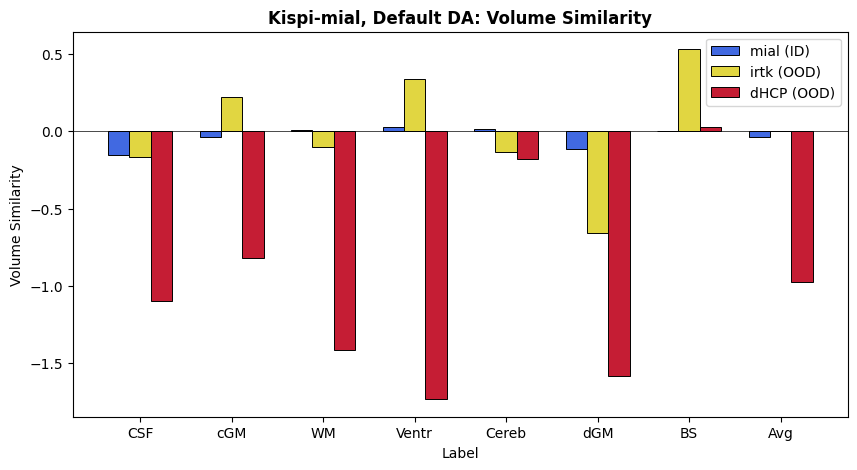
\includegraphics[width=0.8\textwidth]{figures/mial_default_VS.png}\\
    \vspace{10pt}
    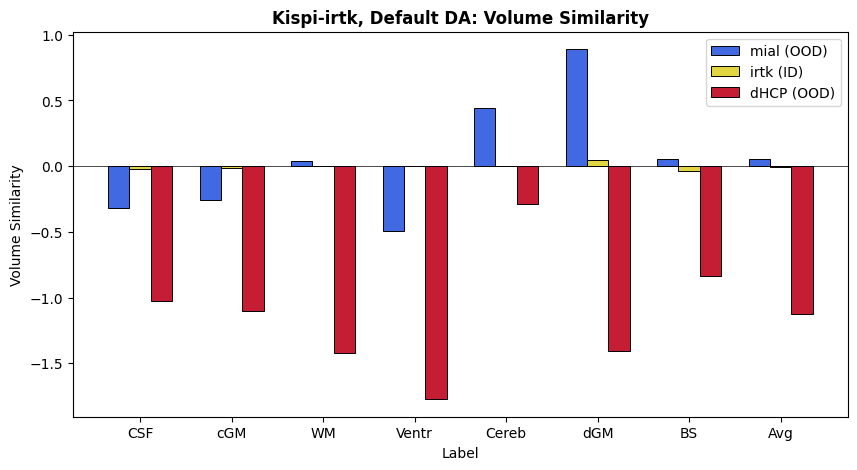
\includegraphics[width=0.8\textwidth]{figures/irtk_default_VS.png}\\
    \vspace{10pt}
    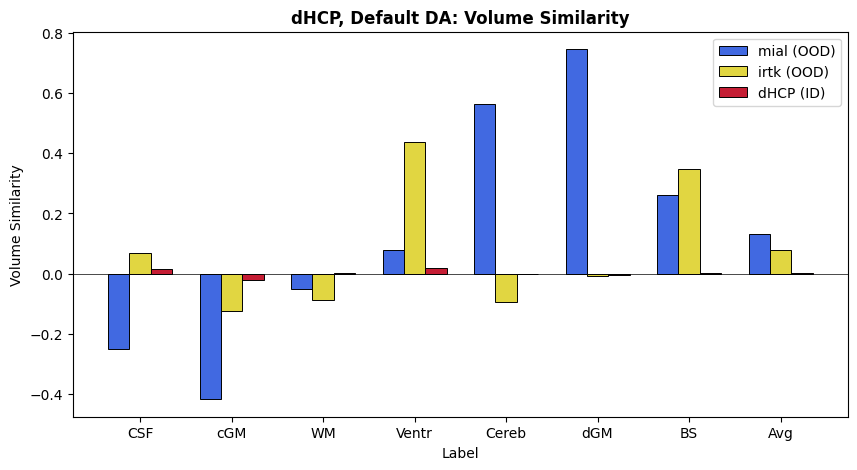
\includegraphics[width=0.8\textwidth]{figures/dHCP_default_VS.png}
    \caption{Volume similarity across datasets and labels for the nnU-Net default DA (baseline model). From top to bottom: training on Kispi-mial, on Kispi-irtk, and on dHCP.}
    \label{fig:default_VS}
\end{figure}

\begin{figure}[htbp]
    \centering
    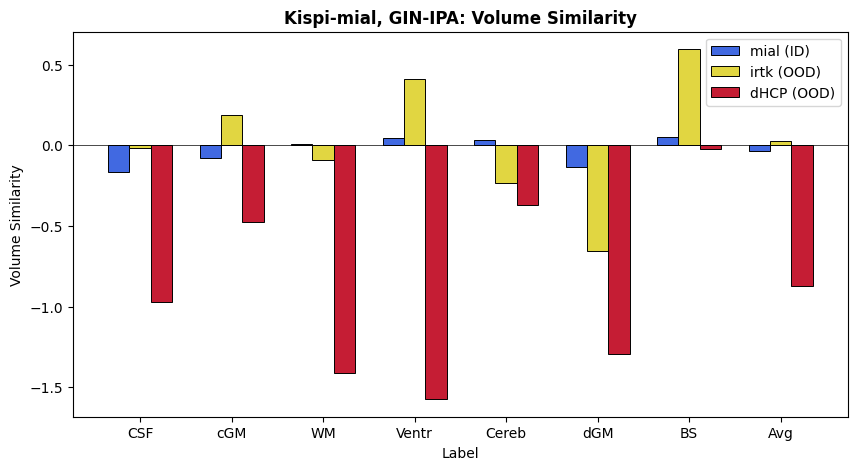
\includegraphics[width=0.8\textwidth]{figures/mial_ginipa_VS.png}\\
    \vspace{10pt}
    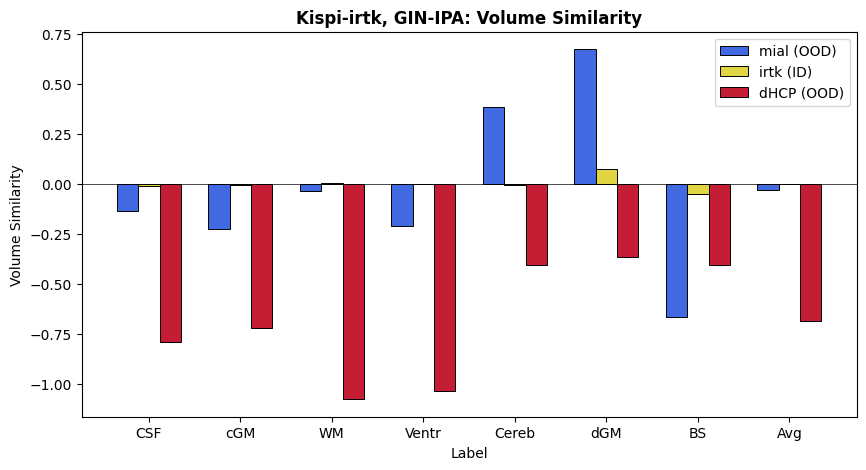
\includegraphics[width=0.8\textwidth]{figures/irtk_ginipa_VS.png}\\
    \vspace{10pt}
    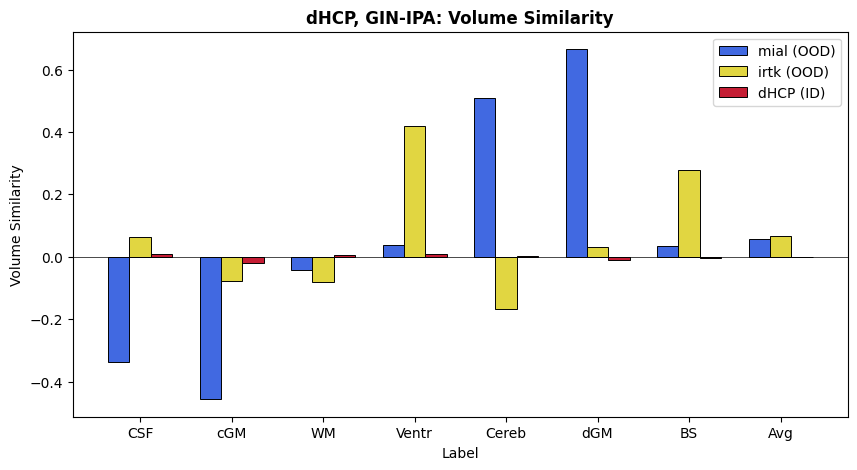
\includegraphics[width=0.8\textwidth]{figures/dHCP_ginipa_VS.png}
    \caption{Volume similarity across datasets and labels for the GIN-IPA DA model. From top to bottom: training on Kispi-mial, on Kispi-irtk, and on dHCP.}
    \label{fig:ginipa_VS}
\end{figure}

\begin{figure}[htbp]
    \centering
    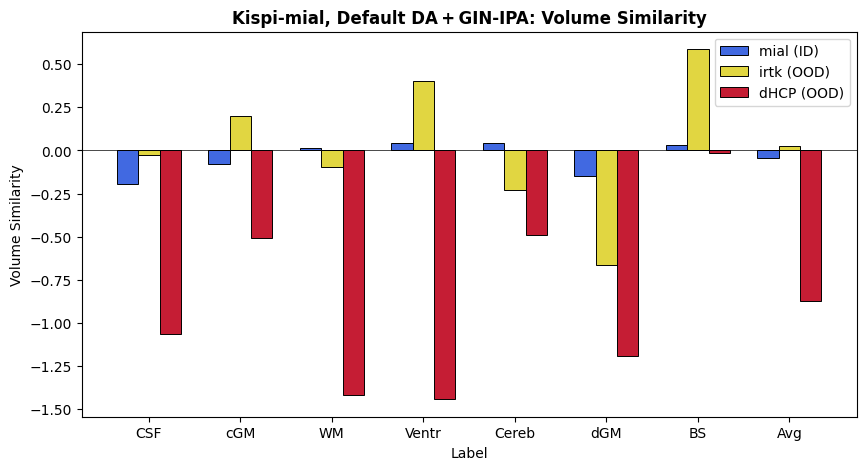
\includegraphics[width=0.8\textwidth]{figures/mial_both_VS.png}\\
    \vspace{10pt}
    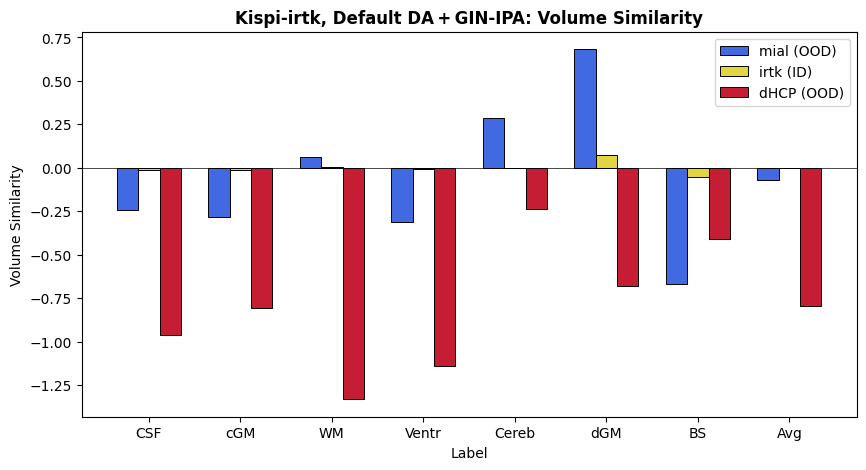
\includegraphics[width=0.8\textwidth]{figures/irtk_both_VS.png}\\
    \vspace{10pt}
    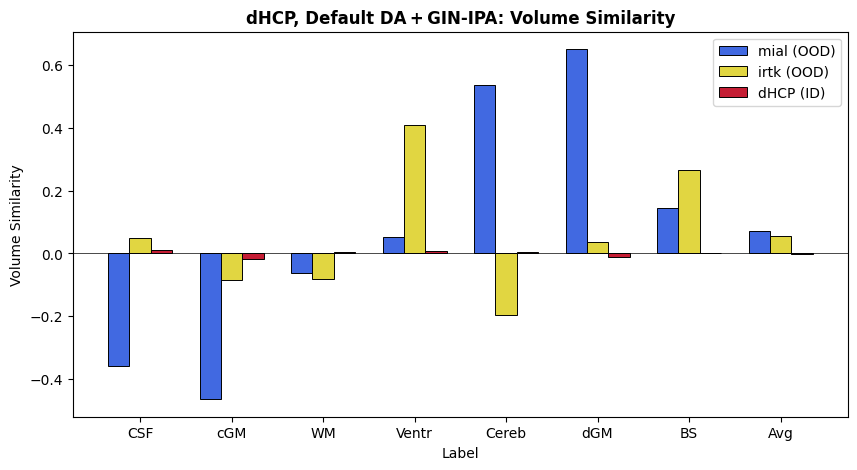
\includegraphics[width=0.8\textwidth]{figures/dHCP_both_VS.png}
    \caption{Volume similarity across datasets and labels for the combined DA (default\,+\,GIN-IPA) model. From top to bottom: training on Kispi-mial, on Kispi-irtk, and on dHCP.}
    \label{fig:both_VS}
\end{figure}

\begin{figure}[htbp]
    \centering
    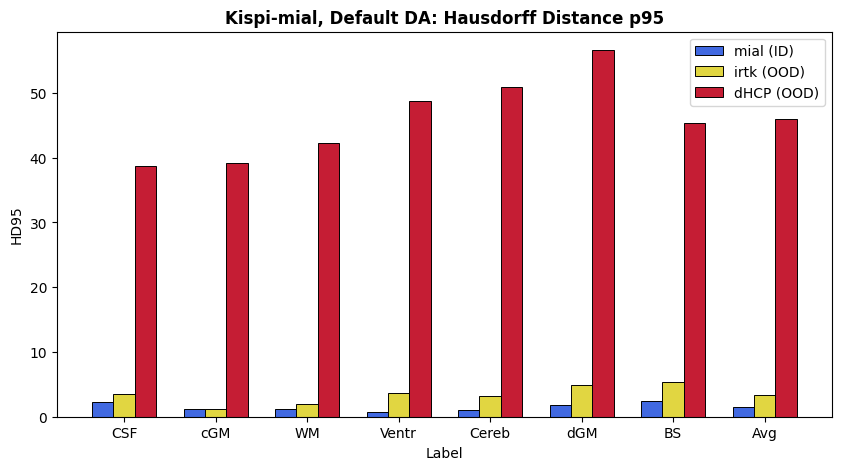
\includegraphics[width=0.8\textwidth]{figures/mial_default_HD.png}\\
    \vspace{2pt}
    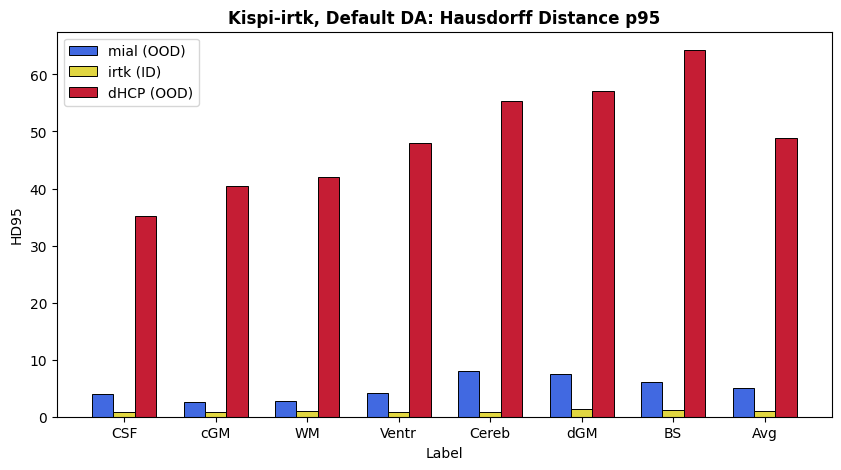
\includegraphics[width=0.8\textwidth]{figures/irtk_default_HD.png}\\
    \vspace{2pt}
    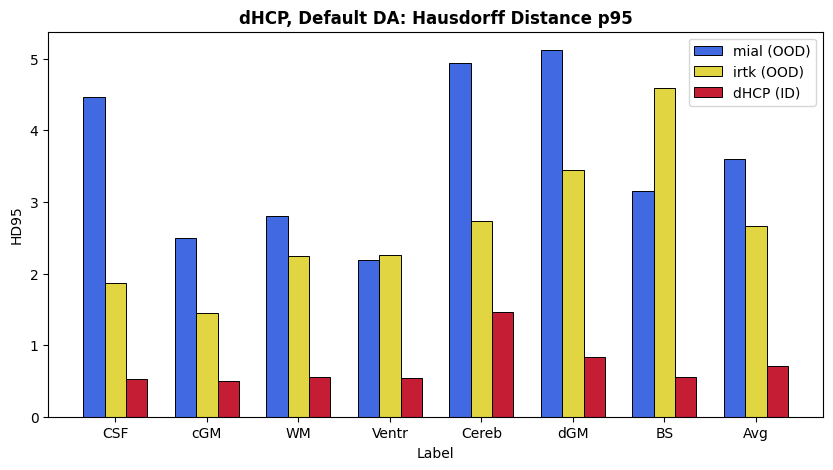
\includegraphics[width=0.8\textwidth]{figures/dHCP_default_HD.png}
    \caption{Hausdorff distance 95\th percentile across datasets and labels for the nnU-Net default DA (baseline model). From top to bottom: training on Kispi-mial, on Kispi-irtk, and on dHCP.}
    \label{fig:default_HD}
\end{figure}

\begin{figure}[htbp]
    \centering
    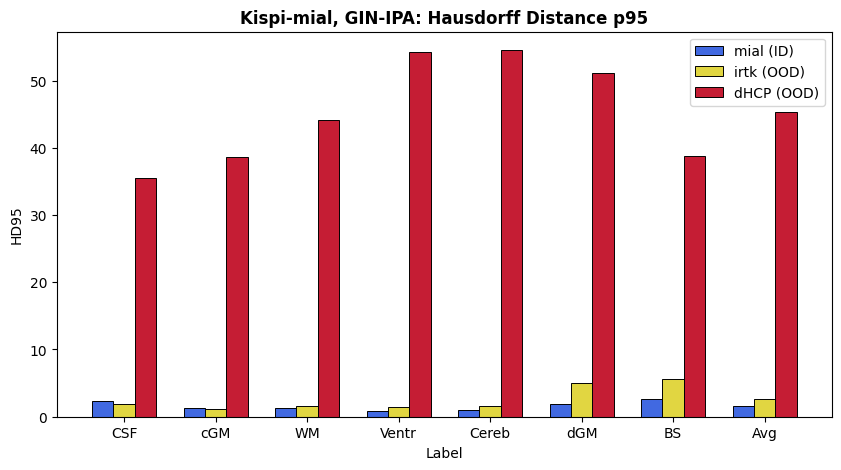
\includegraphics[width=0.8\textwidth]{figures/mial_ginipa_HD.png}\\
    \vspace{5pt}
    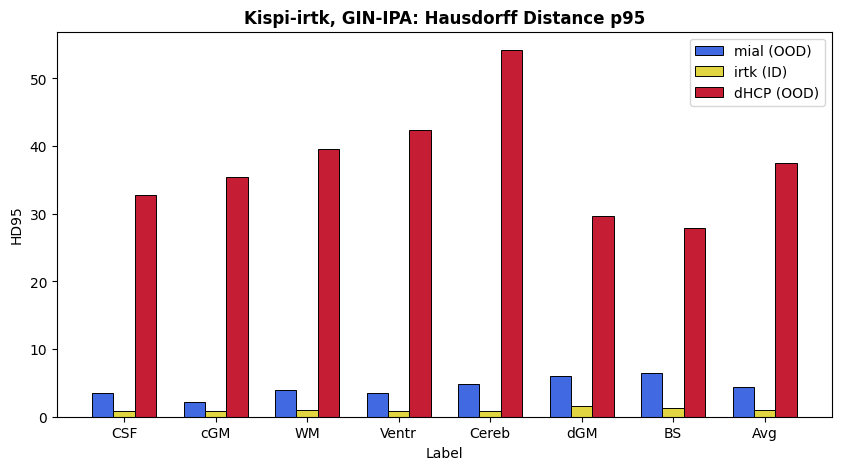
\includegraphics[width=0.8\textwidth]{figures/irtk_ginipa_HD.png}\\
    \vspace{5pt}
    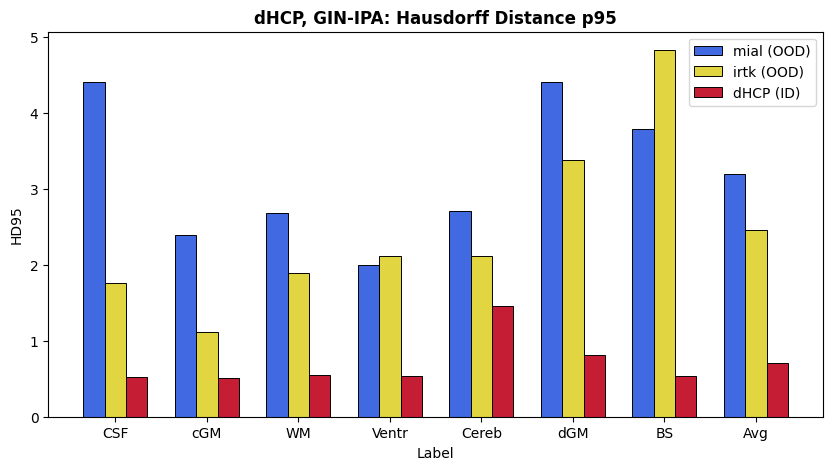
\includegraphics[width=0.8\textwidth]{figures/dHCP_ginipa_HD.png}
    \caption{Hausdorff distance 95\th percentile across datasets and labels for the GIN-IPA DA model. From top to bottom: training on Kispi-mial, on Kispi-irtk, and on dHCP.}
    \label{fig:ginipa_HD}
\end{figure}

\begin{figure}[htbp]
    \centering
    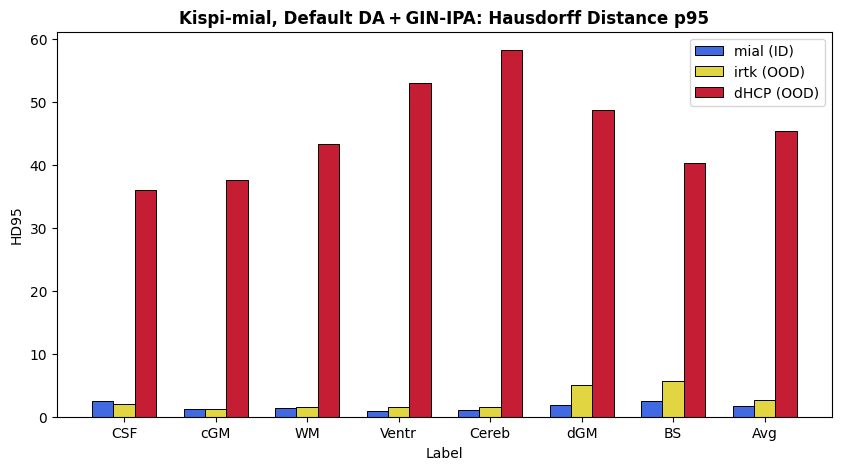
\includegraphics[width=0.8\textwidth]{figures/mial_both_HD.png}\\
    \vspace{2pt}
    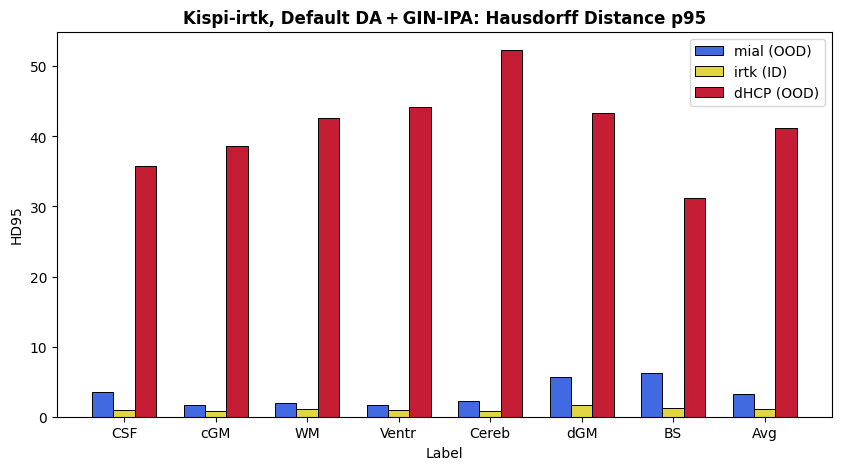
\includegraphics[width=0.8\textwidth]{figures/irtk_both_HD.png}\\
    \vspace{2pt}
    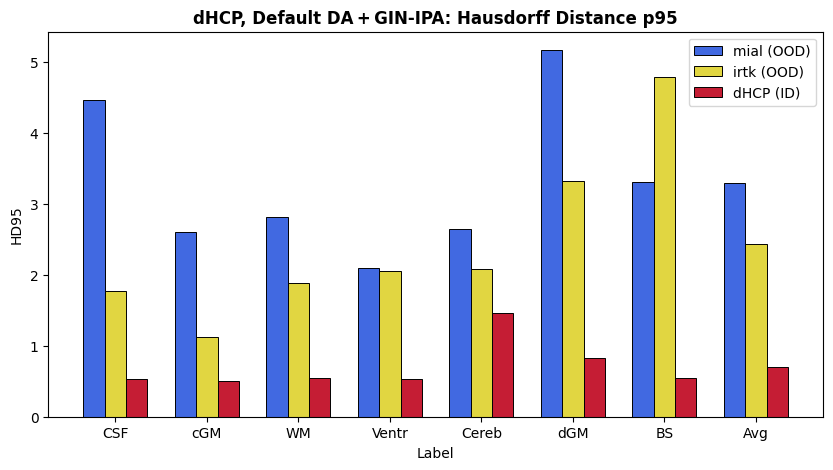
\includegraphics[width=0.8\textwidth]{figures/dHCP_both_HD.png}
    \caption{Hausdorff distance 95\th percentile across datasets and labels for the combined DA (default\,+\,GIN-IPA) model. From top to bottom: training on Kispi-mial, on Kispi-irtk, and on dHCP.}
    \label{fig:both_HD}
\end{figure}

\section{Comparison of Model Performances}
In the plots below are shown the KDE plots related to the comparison between the nnU-Net default DA (baseline model) and the GIN-IPA augmentation model. The plots represent the volume similarity (Fig.\,\ref{fig:1_irtk_dhcp_VS}) and the Hausdorff distance 95\th percentile (Fig.\,\ref{fig:1_irtk_dhcp_HD}) across each label and globally, from models trained on Kispi-irtk and inferring on dHCP. The plots regarding the Dice score are in Section \ref{sec:ComparisonOfModelPerformances}.

\begin{figure}[htbp]
    \centering
    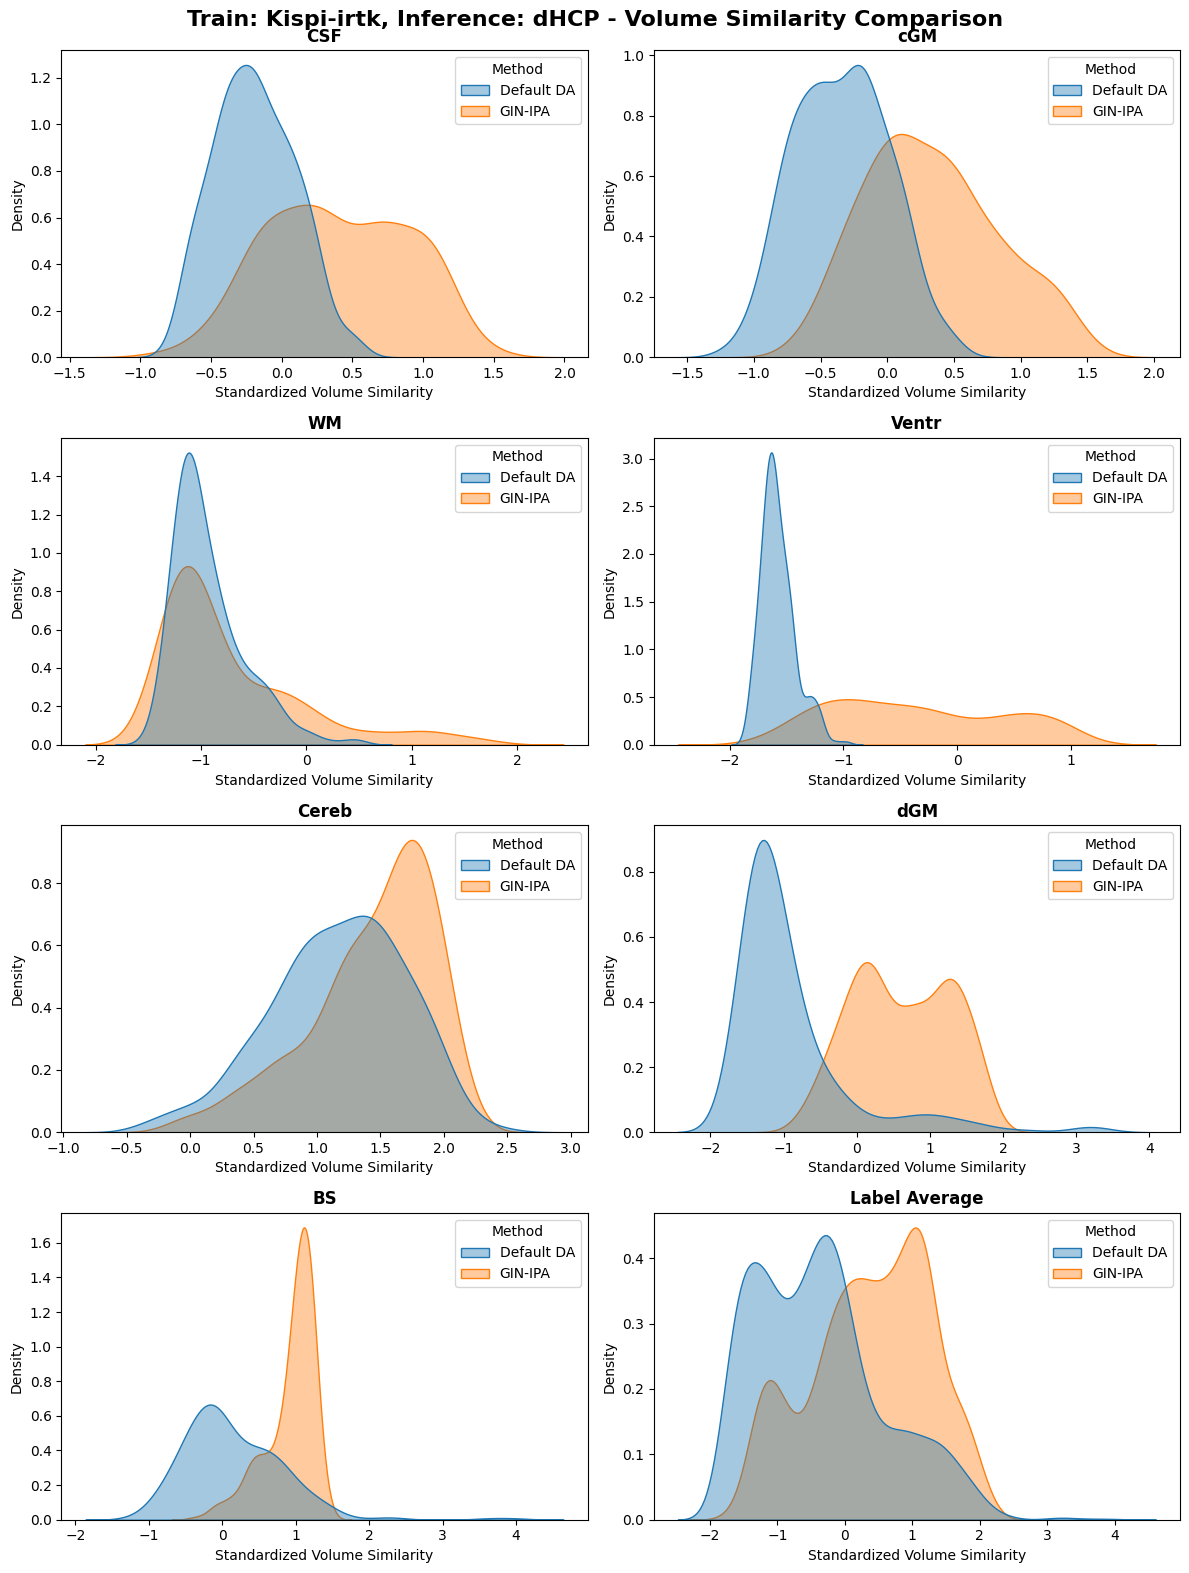
\includegraphics[width=0.95\textwidth]{figures/1_irtk-dhcp_VS.png}
    \caption{Baseline vs.\ GIN-IPA: KDE plots of the volume similarity across each label and globally, from models trained on Kispi-irtk and inferring on dHCP.}
    \label{fig:1_irtk_dhcp_VS}
\end{figure}

\begin{figure}[htbp]
    \centering
    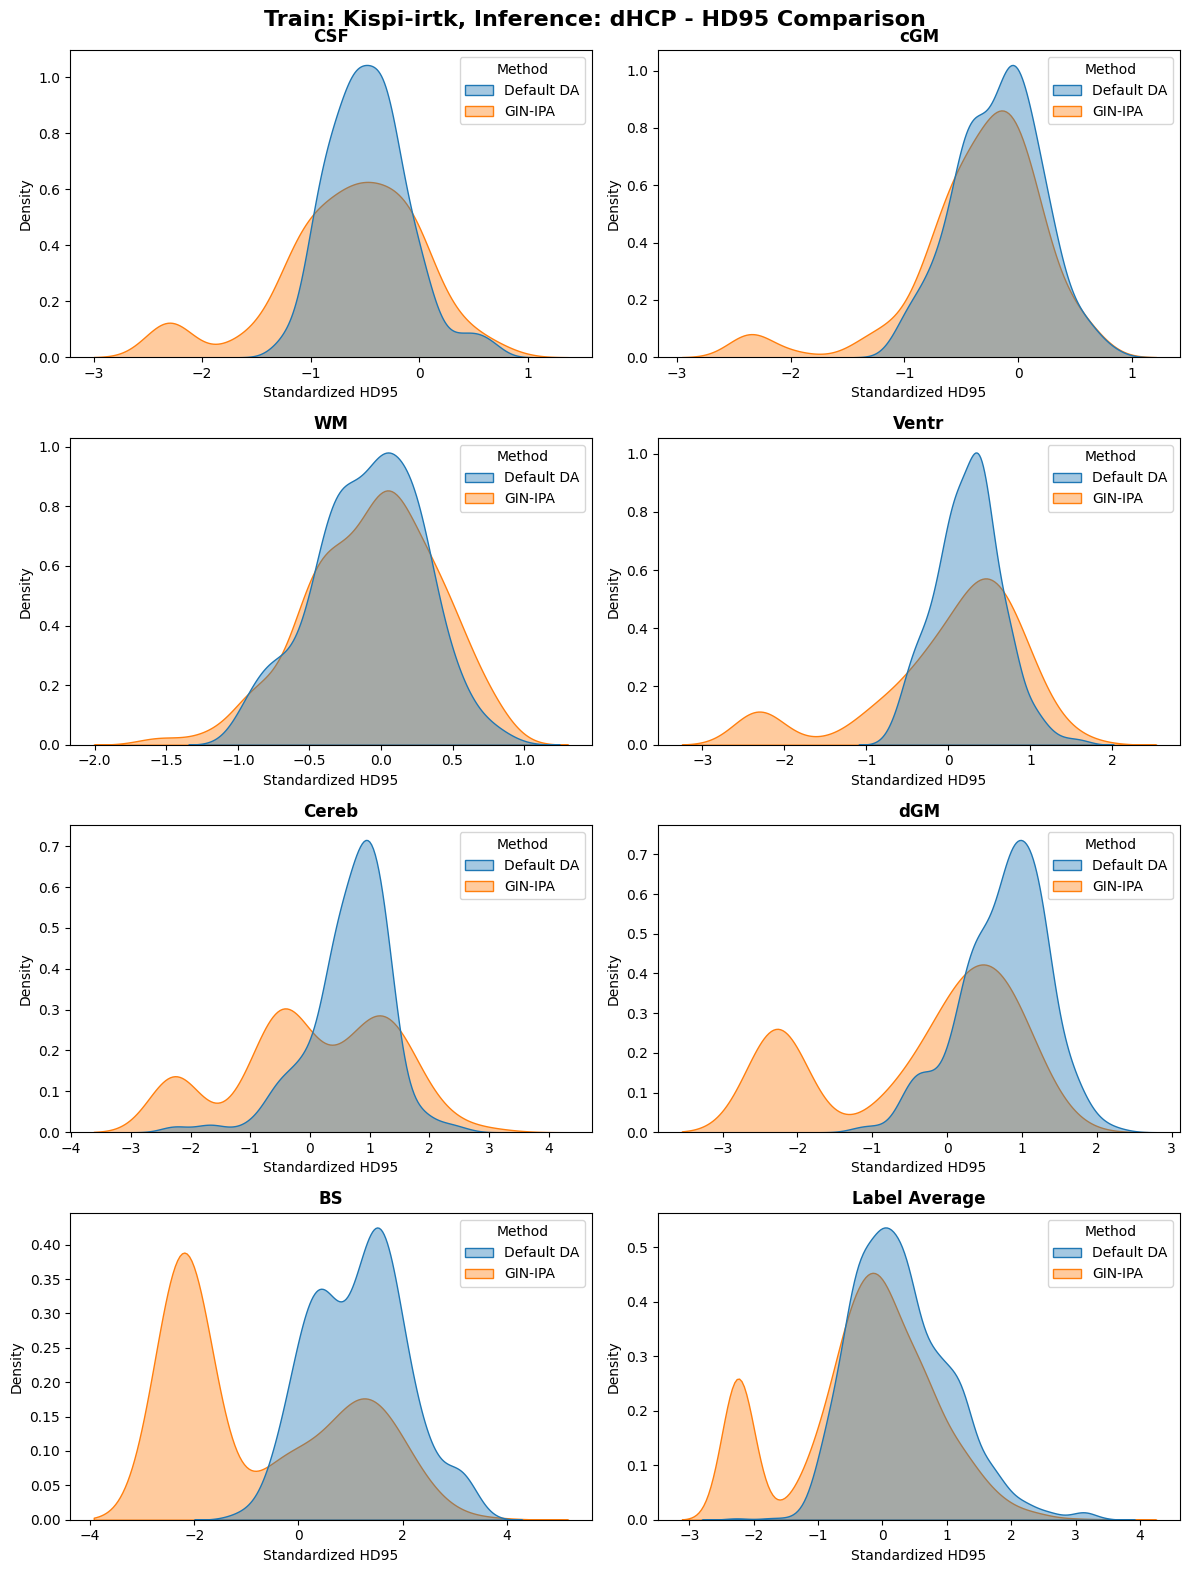
\includegraphics[width=0.95\textwidth]{figures/1_irtk-dhcp_HD.png}
    \caption{Baseline vs.\ GIN-IPA: KDE plots of the Hausdorff distance 95\th percentile across each label and globally, from models trained on Kispi-irtk and inferring on dHCP.}
    \label{fig:1_irtk_dhcp_HD}
\end{figure}
